% Created by tikzDevice version 0.10.1 on 2018-01-24 12:52:14
% !TEX encoding = UTF-8 Unicode
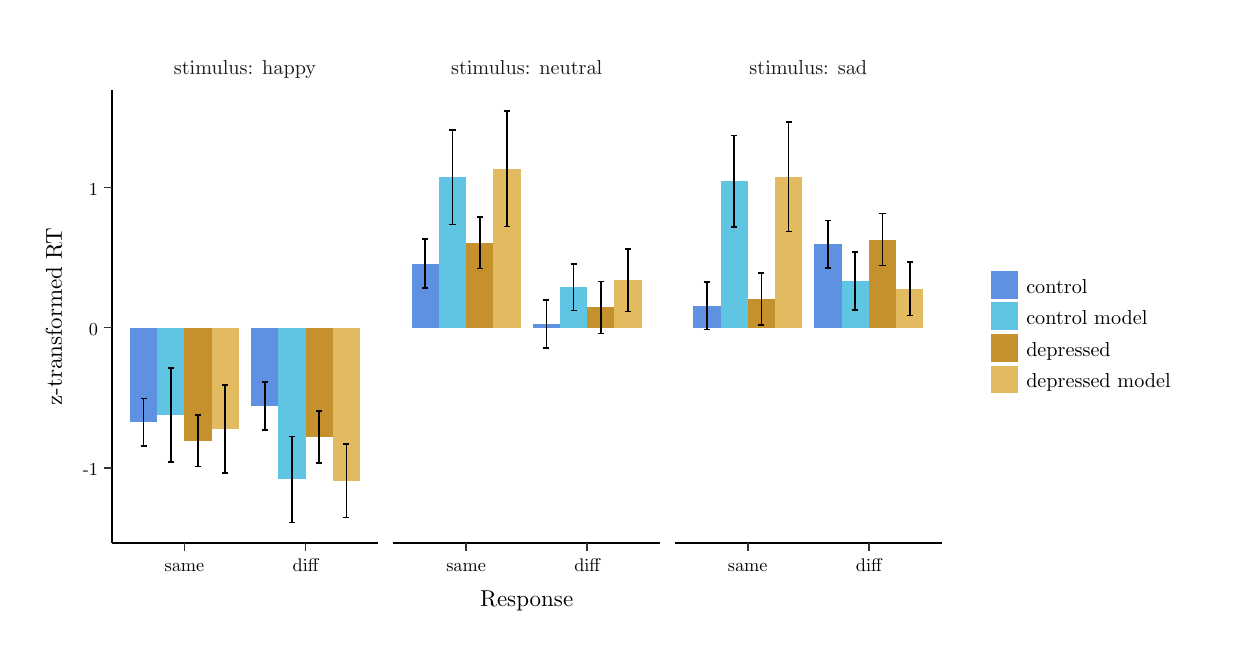
\begin{tikzpicture}[x=1pt,y=1pt]
\definecolor{fillColor}{RGB}{255,255,255}
\path[use as bounding box,fill=fillColor,fill opacity=0.00] (0,0) rectangle (433.62,216.81);
\begin{scope}
\path[clip] (  0.00,  0.00) rectangle (433.62,216.81);
\definecolor{drawColor}{RGB}{255,255,255}
\definecolor{fillColor}{RGB}{255,255,255}

\path[draw=drawColor,line width= 0.6pt,line join=round,line cap=round,fill=fillColor] (  0.00,  0.00) rectangle (433.62,216.81);
\end{scope}
\begin{scope}
\path[clip] ( 30.40, 30.56) rectangle (126.67,194.25);
\definecolor{fillColor}{RGB}{255,255,255}

\path[fill=fillColor] ( 30.40, 30.56) rectangle (126.67,194.25);
\definecolor{fillColor}{RGB}{226,186,95}

\path[fill=fillColor] ( 66.50, 71.75) rectangle ( 76.34,108.42);
\definecolor{fillColor}{RGB}{196,145,45}

\path[fill=fillColor] ( 56.65, 67.55) rectangle ( 66.50,108.42);
\definecolor{fillColor}{RGB}{95,197,226}

\path[fill=fillColor] ( 46.81, 76.75) rectangle ( 56.65,108.42);
\definecolor{fillColor}{RGB}{95,145,226}

\path[fill=fillColor] ( 36.96, 74.16) rectangle ( 46.81,108.42);
\definecolor{fillColor}{RGB}{226,186,95}

\path[fill=fillColor] (110.26, 53.10) rectangle (120.11,108.42);
\definecolor{fillColor}{RGB}{196,145,45}

\path[fill=fillColor] (100.41, 68.87) rectangle (110.26,108.42);
\definecolor{fillColor}{RGB}{95,197,226}

\path[fill=fillColor] ( 90.57, 53.56) rectangle (100.41,108.42);
\definecolor{fillColor}{RGB}{95,145,226}

\path[fill=fillColor] ( 80.72, 80.04) rectangle ( 90.57,108.42);
\definecolor{drawColor}{RGB}{0,0,0}

\path[draw=drawColor,line width= 0.6pt,line join=round] ( 70.33, 87.58) --
	( 72.52, 87.58);

\path[draw=drawColor,line width= 0.6pt,line join=round] ( 71.42, 87.58) --
	( 71.42, 55.91);

\path[draw=drawColor,line width= 0.6pt,line join=round] ( 70.33, 55.91) --
	( 72.52, 55.91);

\path[draw=drawColor,line width= 0.6pt,line join=round] ( 60.48, 76.92) --
	( 62.67, 76.92);

\path[draw=drawColor,line width= 0.6pt,line join=round] ( 61.58, 76.92) --
	( 61.58, 58.19);

\path[draw=drawColor,line width= 0.6pt,line join=round] ( 60.48, 58.19) --
	( 62.67, 58.19);

\path[draw=drawColor,line width= 0.6pt,line join=round] ( 50.63, 93.74) --
	( 52.82, 93.74);

\path[draw=drawColor,line width= 0.6pt,line join=round] ( 51.73, 93.74) --
	( 51.73, 59.75);

\path[draw=drawColor,line width= 0.6pt,line join=round] ( 50.63, 59.75) --
	( 52.82, 59.75);

\path[draw=drawColor,line width= 0.6pt,line join=round] ( 40.79, 82.77) --
	( 42.98, 82.77);

\path[draw=drawColor,line width= 0.6pt,line join=round] ( 41.88, 82.77) --
	( 41.88, 65.55);

\path[draw=drawColor,line width= 0.6pt,line join=round] ( 40.79, 65.55) --
	( 42.98, 65.55);

\path[draw=drawColor,line width= 0.6pt,line join=round] (114.09, 66.35) --
	(116.28, 66.35);

\path[draw=drawColor,line width= 0.6pt,line join=round] (115.18, 66.35) --
	(115.18, 39.85);

\path[draw=drawColor,line width= 0.6pt,line join=round] (114.09, 39.85) --
	(116.28, 39.85);

\path[draw=drawColor,line width= 0.6pt,line join=round] (104.24, 78.24) --
	(106.43, 78.24);

\path[draw=drawColor,line width= 0.6pt,line join=round] (105.34, 78.24) --
	(105.34, 59.51);

\path[draw=drawColor,line width= 0.6pt,line join=round] (104.24, 59.51) --
	(106.43, 59.51);

\path[draw=drawColor,line width= 0.6pt,line join=round] ( 94.40, 69.13) --
	( 96.58, 69.13);

\path[draw=drawColor,line width= 0.6pt,line join=round] ( 95.49, 69.13) --
	( 95.49, 38.00);

\path[draw=drawColor,line width= 0.6pt,line join=round] ( 94.40, 38.00) --
	( 96.58, 38.00);

\path[draw=drawColor,line width= 0.6pt,line join=round] ( 84.55, 88.67) --
	( 86.74, 88.67);

\path[draw=drawColor,line width= 0.6pt,line join=round] ( 85.64, 88.67) --
	( 85.64, 71.42);

\path[draw=drawColor,line width= 0.6pt,line join=round] ( 84.55, 71.42) --
	( 86.74, 71.42);
\end{scope}
\begin{scope}
\path[clip] (132.17, 30.56) rectangle (228.44,194.25);
\definecolor{fillColor}{RGB}{255,255,255}

\path[fill=fillColor] (132.17, 30.56) rectangle (228.44,194.25);
\definecolor{fillColor}{RGB}{226,186,95}

\path[fill=fillColor] (168.27,108.42) rectangle (178.12,165.91);
\definecolor{fillColor}{RGB}{196,145,45}

\path[fill=fillColor] (158.43,108.42) rectangle (168.27,139.13);
\definecolor{fillColor}{RGB}{95,197,226}

\path[fill=fillColor] (148.58,108.42) rectangle (158.43,162.76);
\definecolor{fillColor}{RGB}{95,145,226}

\path[fill=fillColor] (138.73,108.42) rectangle (148.58,131.52);
\definecolor{fillColor}{RGB}{226,186,95}

\path[fill=fillColor] (212.03,108.42) rectangle (221.88,125.56);
\definecolor{fillColor}{RGB}{196,145,45}

\path[fill=fillColor] (202.19,108.42) rectangle (212.03,115.71);
\definecolor{fillColor}{RGB}{95,197,226}

\path[fill=fillColor] (192.34,108.42) rectangle (202.19,123.01);
\definecolor{fillColor}{RGB}{95,145,226}

\path[fill=fillColor] (182.49,108.42) rectangle (192.34,109.74);
\definecolor{drawColor}{RGB}{0,0,0}

\path[draw=drawColor,line width= 0.6pt,line join=round] (172.10,186.81) --
	(174.29,186.81);

\path[draw=drawColor,line width= 0.6pt,line join=round] (173.20,186.81) --
	(173.20,145.01);

\path[draw=drawColor,line width= 0.6pt,line join=round] (172.10,145.01) --
	(174.29,145.01);

\path[draw=drawColor,line width= 0.6pt,line join=round] (162.25,148.49) --
	(164.44,148.49);

\path[draw=drawColor,line width= 0.6pt,line join=round] (163.35,148.49) --
	(163.35,129.76);

\path[draw=drawColor,line width= 0.6pt,line join=round] (162.25,129.76) --
	(164.44,129.76);

\path[draw=drawColor,line width= 0.6pt,line join=round] (152.41,179.79) --
	(154.60,179.79);

\path[draw=drawColor,line width= 0.6pt,line join=round] (153.50,179.79) --
	(153.50,145.72);

\path[draw=drawColor,line width= 0.6pt,line join=round] (152.41,145.72) --
	(154.60,145.72);

\path[draw=drawColor,line width= 0.6pt,line join=round] (142.56,140.35) --
	(144.75,140.35);

\path[draw=drawColor,line width= 0.6pt,line join=round] (143.66,140.35) --
	(143.66,122.69);

\path[draw=drawColor,line width= 0.6pt,line join=round] (142.56,122.69) --
	(144.75,122.69);

\path[draw=drawColor,line width= 0.6pt,line join=round] (215.86,136.84) --
	(218.05,136.84);

\path[draw=drawColor,line width= 0.6pt,line join=round] (216.96,136.84) --
	(216.96,114.29);

\path[draw=drawColor,line width= 0.6pt,line join=round] (215.86,114.29) --
	(218.05,114.29);

\path[draw=drawColor,line width= 0.6pt,line join=round] (206.02,125.10) --
	(208.20,125.10);

\path[draw=drawColor,line width= 0.6pt,line join=round] (207.11,125.10) --
	(207.11,106.32);

\path[draw=drawColor,line width= 0.6pt,line join=round] (206.02,106.32) --
	(208.20,106.32);

\path[draw=drawColor,line width= 0.6pt,line join=round] (196.17,131.45) --
	(198.36,131.45);

\path[draw=drawColor,line width= 0.6pt,line join=round] (197.26,131.45) --
	(197.26,114.57);

\path[draw=drawColor,line width= 0.6pt,line join=round] (196.17,114.57) --
	(198.36,114.57);

\path[draw=drawColor,line width= 0.6pt,line join=round] (186.32,118.35) --
	(188.51,118.35);

\path[draw=drawColor,line width= 0.6pt,line join=round] (187.42,118.35) --
	(187.42,101.14);

\path[draw=drawColor,line width= 0.6pt,line join=round] (186.32,101.14) --
	(188.51,101.14);
\end{scope}
\begin{scope}
\path[clip] (233.94, 30.56) rectangle (330.22,194.25);
\definecolor{fillColor}{RGB}{255,255,255}

\path[fill=fillColor] (233.94, 30.56) rectangle (330.22,194.25);
\definecolor{fillColor}{RGB}{226,186,95}

\path[fill=fillColor] (270.05,108.42) rectangle (279.89,162.94);
\definecolor{fillColor}{RGB}{196,145,45}

\path[fill=fillColor] (260.20,108.42) rectangle (270.05,118.67);
\definecolor{fillColor}{RGB}{95,197,226}

\path[fill=fillColor] (250.35,108.42) rectangle (260.20,161.32);
\definecolor{fillColor}{RGB}{95,145,226}

\path[fill=fillColor] (240.51,108.42) rectangle (250.35,116.31);
\definecolor{fillColor}{RGB}{226,186,95}

\path[fill=fillColor] (313.81,108.42) rectangle (323.65,122.43);
\definecolor{fillColor}{RGB}{196,145,45}

\path[fill=fillColor] (303.96,108.42) rectangle (313.81,140.25);
\definecolor{fillColor}{RGB}{95,197,226}

\path[fill=fillColor] (294.11,108.42) rectangle (303.96,125.26);
\definecolor{fillColor}{RGB}{95,145,226}

\path[fill=fillColor] (284.27,108.42) rectangle (294.11,138.53);
\definecolor{drawColor}{RGB}{0,0,0}

\path[draw=drawColor,line width= 0.6pt,line join=round] (273.87,182.75) --
	(276.06,182.75);

\path[draw=drawColor,line width= 0.6pt,line join=round] (274.97,182.75) --
	(274.97,143.13);

\path[draw=drawColor,line width= 0.6pt,line join=round] (273.87,143.13) --
	(276.06,143.13);

\path[draw=drawColor,line width= 0.6pt,line join=round] (264.03,128.04) --
	(266.22,128.04);

\path[draw=drawColor,line width= 0.6pt,line join=round] (265.12,128.04) --
	(265.12,109.30);

\path[draw=drawColor,line width= 0.6pt,line join=round] (264.03,109.30) --
	(266.22,109.30);

\path[draw=drawColor,line width= 0.6pt,line join=round] (254.18,177.81) --
	(256.37,177.81);

\path[draw=drawColor,line width= 0.6pt,line join=round] (255.28,177.81) --
	(255.28,144.83);

\path[draw=drawColor,line width= 0.6pt,line join=round] (254.18,144.83) --
	(256.37,144.83);

\path[draw=drawColor,line width= 0.6pt,line join=round] (244.34,124.92) --
	(246.52,124.92);

\path[draw=drawColor,line width= 0.6pt,line join=round] (245.43,124.92) --
	(245.43,107.70);

\path[draw=drawColor,line width= 0.6pt,line join=round] (244.34,107.70) --
	(246.52,107.70);

\path[draw=drawColor,line width= 0.6pt,line join=round] (317.64,132.06) --
	(319.82,132.06);

\path[draw=drawColor,line width= 0.6pt,line join=round] (318.73,132.06) --
	(318.73,112.80);

\path[draw=drawColor,line width= 0.6pt,line join=round] (317.64,112.80) --
	(319.82,112.80);

\path[draw=drawColor,line width= 0.6pt,line join=round] (307.79,149.63) --
	(309.98,149.63);

\path[draw=drawColor,line width= 0.6pt,line join=round] (308.88,149.63) --
	(308.88,130.86);

\path[draw=drawColor,line width= 0.6pt,line join=round] (307.79,130.86) --
	(309.98,130.86);

\path[draw=drawColor,line width= 0.6pt,line join=round] (297.94,135.74) --
	(300.13,135.74);

\path[draw=drawColor,line width= 0.6pt,line join=round] (299.04,135.74) --
	(299.04,114.78);

\path[draw=drawColor,line width= 0.6pt,line join=round] (297.94,114.78) --
	(300.13,114.78);

\path[draw=drawColor,line width= 0.6pt,line join=round] (288.10,147.13) --
	(290.29,147.13);

\path[draw=drawColor,line width= 0.6pt,line join=round] (289.19,147.13) --
	(289.19,129.92);

\path[draw=drawColor,line width= 0.6pt,line join=round] (288.10,129.92) --
	(290.29,129.92);
\end{scope}
\begin{scope}
\path[clip] ( 30.40,194.25) rectangle (126.67,211.31);
\definecolor{drawColor}{RGB}{255,255,255}
\definecolor{fillColor}{RGB}{255,255,255}

\path[draw=drawColor,line width= 1.1pt,line join=round,line cap=round,fill=fillColor] ( 30.40,194.25) rectangle (126.67,211.31);
\definecolor{drawColor}{gray}{0.10}

\node[text=drawColor,anchor=base,inner sep=0pt, outer sep=0pt, scale=  0.73] at ( 78.53,199.75) {stimulus: happy};
\end{scope}
\begin{scope}
\path[clip] (132.17,194.25) rectangle (228.44,211.31);
\definecolor{drawColor}{RGB}{255,255,255}
\definecolor{fillColor}{RGB}{255,255,255}

\path[draw=drawColor,line width= 1.1pt,line join=round,line cap=round,fill=fillColor] (132.17,194.25) rectangle (228.44,211.31);
\definecolor{drawColor}{gray}{0.10}

\node[text=drawColor,anchor=base,inner sep=0pt, outer sep=0pt, scale=  0.73] at (180.31,199.75) {stimulus: neutral};
\end{scope}
\begin{scope}
\path[clip] (233.94,194.25) rectangle (330.22,211.31);
\definecolor{drawColor}{RGB}{255,255,255}
\definecolor{fillColor}{RGB}{255,255,255}

\path[draw=drawColor,line width= 1.1pt,line join=round,line cap=round,fill=fillColor] (233.94,194.25) rectangle (330.22,211.31);
\definecolor{drawColor}{gray}{0.10}

\node[text=drawColor,anchor=base,inner sep=0pt, outer sep=0pt, scale=  0.73] at (282.08,199.75) {stimulus: sad};
\end{scope}
\begin{scope}
\path[clip] (  0.00,  0.00) rectangle (433.62,216.81);
\definecolor{drawColor}{RGB}{0,0,0}

\path[draw=drawColor,line width= 0.6pt,line join=round] ( 30.40, 30.56) --
	(126.67, 30.56);
\end{scope}
\begin{scope}
\path[clip] (  0.00,  0.00) rectangle (433.62,216.81);
\definecolor{drawColor}{gray}{0.20}

\path[draw=drawColor,line width= 0.6pt,line join=round] ( 56.65, 27.81) --
	( 56.65, 30.56);

\path[draw=drawColor,line width= 0.6pt,line join=round] (100.41, 27.81) --
	(100.41, 30.56);
\end{scope}
\begin{scope}
\path[clip] (  0.00,  0.00) rectangle (433.62,216.81);
\definecolor{drawColor}{RGB}{0,0,0}

\node[text=drawColor,anchor=base,inner sep=0pt, outer sep=0pt, scale=  0.66] at ( 56.65, 20.15) {same};

\node[text=drawColor,anchor=base,inner sep=0pt, outer sep=0pt, scale=  0.66] at (100.41, 20.15) {diff};
\end{scope}
\begin{scope}
\path[clip] (  0.00,  0.00) rectangle (433.62,216.81);
\definecolor{drawColor}{RGB}{0,0,0}

\path[draw=drawColor,line width= 0.6pt,line join=round] (132.17, 30.56) --
	(228.44, 30.56);
\end{scope}
\begin{scope}
\path[clip] (  0.00,  0.00) rectangle (433.62,216.81);
\definecolor{drawColor}{gray}{0.20}

\path[draw=drawColor,line width= 0.6pt,line join=round] (158.43, 27.81) --
	(158.43, 30.56);

\path[draw=drawColor,line width= 0.6pt,line join=round] (202.19, 27.81) --
	(202.19, 30.56);
\end{scope}
\begin{scope}
\path[clip] (  0.00,  0.00) rectangle (433.62,216.81);
\definecolor{drawColor}{RGB}{0,0,0}

\node[text=drawColor,anchor=base,inner sep=0pt, outer sep=0pt, scale=  0.66] at (158.43, 20.15) {same};

\node[text=drawColor,anchor=base,inner sep=0pt, outer sep=0pt, scale=  0.66] at (202.19, 20.15) {diff};
\end{scope}
\begin{scope}
\path[clip] (  0.00,  0.00) rectangle (433.62,216.81);
\definecolor{drawColor}{RGB}{0,0,0}

\path[draw=drawColor,line width= 0.6pt,line join=round] (233.94, 30.56) --
	(330.22, 30.56);
\end{scope}
\begin{scope}
\path[clip] (  0.00,  0.00) rectangle (433.62,216.81);
\definecolor{drawColor}{gray}{0.20}

\path[draw=drawColor,line width= 0.6pt,line join=round] (260.20, 27.81) --
	(260.20, 30.56);

\path[draw=drawColor,line width= 0.6pt,line join=round] (303.96, 27.81) --
	(303.96, 30.56);
\end{scope}
\begin{scope}
\path[clip] (  0.00,  0.00) rectangle (433.62,216.81);
\definecolor{drawColor}{RGB}{0,0,0}

\node[text=drawColor,anchor=base,inner sep=0pt, outer sep=0pt, scale=  0.66] at (260.20, 20.15) {same};

\node[text=drawColor,anchor=base,inner sep=0pt, outer sep=0pt, scale=  0.66] at (303.96, 20.15) {diff};
\end{scope}
\begin{scope}
\path[clip] (  0.00,  0.00) rectangle (433.62,216.81);
\definecolor{drawColor}{RGB}{0,0,0}

\path[draw=drawColor,line width= 0.6pt,line join=round] ( 30.40, 30.56) --
	( 30.40,194.25);
\end{scope}
\begin{scope}
\path[clip] (  0.00,  0.00) rectangle (433.62,216.81);
\definecolor{drawColor}{RGB}{0,0,0}

\node[text=drawColor,anchor=base east,inner sep=0pt, outer sep=0pt, scale=  0.66] at ( 25.45, 55.06) {-1};

\node[text=drawColor,anchor=base east,inner sep=0pt, outer sep=0pt, scale=  0.66] at ( 25.45,105.70) {0};

\node[text=drawColor,anchor=base east,inner sep=0pt, outer sep=0pt, scale=  0.66] at ( 25.45,156.33) {1};
\end{scope}
\begin{scope}
\path[clip] (  0.00,  0.00) rectangle (433.62,216.81);
\definecolor{drawColor}{gray}{0.20}

\path[draw=drawColor,line width= 0.6pt,line join=round] ( 27.65, 57.79) --
	( 30.40, 57.79);

\path[draw=drawColor,line width= 0.6pt,line join=round] ( 27.65,108.42) --
	( 30.40,108.42);

\path[draw=drawColor,line width= 0.6pt,line join=round] ( 27.65,159.06) --
	( 30.40,159.06);
\end{scope}
\begin{scope}
\path[clip] (  0.00,  0.00) rectangle (433.62,216.81);
\definecolor{drawColor}{RGB}{0,0,0}

\node[text=drawColor,anchor=base,inner sep=0pt, outer sep=0pt, scale=  0.83] at (180.31,  7.83) {Response};
\end{scope}
\begin{scope}
\path[clip] (  0.00,  0.00) rectangle (433.62,216.81);
\definecolor{drawColor}{RGB}{0,0,0}

\node[text=drawColor,rotate= 90.00,anchor=base,inner sep=0pt, outer sep=0pt, scale=  0.83] at ( 12.32,112.40) {z-transformed RT};
\end{scope}
\begin{scope}
\path[clip] (  0.00,  0.00) rectangle (433.62,216.81);
\definecolor{fillColor}{RGB}{255,255,255}

\path[fill=fillColor] (341.60, 78.37) rectangle (428.12,146.43);
\end{scope}
\begin{scope}
\path[clip] (  0.00,  0.00) rectangle (433.62,216.81);
\definecolor{fillColor}{RGB}{95,145,226}

\path[fill=fillColor] (348.00,118.92) rectangle (357.96,128.88);
\end{scope}
\begin{scope}
\path[clip] (  0.00,  0.00) rectangle (433.62,216.81);
\definecolor{fillColor}{RGB}{95,197,226}

\path[fill=fillColor] (348.00,107.54) rectangle (357.96,117.50);
\end{scope}
\begin{scope}
\path[clip] (  0.00,  0.00) rectangle (433.62,216.81);
\definecolor{fillColor}{RGB}{196,145,45}

\path[fill=fillColor] (348.00, 96.16) rectangle (357.96,106.11);
\end{scope}
\begin{scope}
\path[clip] (  0.00,  0.00) rectangle (433.62,216.81);
\definecolor{fillColor}{RGB}{226,186,95}

\path[fill=fillColor] (348.00, 84.77) rectangle (357.96, 94.73);
\end{scope}
\begin{scope}
\path[clip] (  0.00,  0.00) rectangle (433.62,216.81);
\definecolor{drawColor}{RGB}{0,0,0}

\node[text=drawColor,anchor=base west,inner sep=0pt, outer sep=0pt, scale=  0.73] at (360.84,120.87) {control};
\end{scope}
\begin{scope}
\path[clip] (  0.00,  0.00) rectangle (433.62,216.81);
\definecolor{drawColor}{RGB}{0,0,0}

\node[text=drawColor,anchor=base west,inner sep=0pt, outer sep=0pt, scale=  0.73] at (360.84,109.49) {control model};
\end{scope}
\begin{scope}
\path[clip] (  0.00,  0.00) rectangle (433.62,216.81);
\definecolor{drawColor}{RGB}{0,0,0}

\node[text=drawColor,anchor=base west,inner sep=0pt, outer sep=0pt, scale=  0.73] at (360.84, 98.10) {depressed};
\end{scope}
\begin{scope}
\path[clip] (  0.00,  0.00) rectangle (433.62,216.81);
\definecolor{drawColor}{RGB}{0,0,0}

\node[text=drawColor,anchor=base west,inner sep=0pt, outer sep=0pt, scale=  0.73] at (360.84, 86.72) {depressed model};
\end{scope}
\end{tikzpicture}
